\chapter{作者项目纪实} \label{app:author-projects}

本书正文中的每一段代码、每一个设计模式、每一次“塑料轮子”决策，都来自作者在真实项目中踩过的坑、烧过的板子和熬过的夜。本附录把那些散落在各章的项目片段重新串起来，形成一个完整的技术成长轨迹——从小学的机器人兴趣班，到大学的竞赛和毕业设计，再到工作后的产品开发。如果你在读正文时好奇“这些方案到底能不能跑”，本附录就是答案。

注：除了早期项目，本附录的项目都可以从我的Gitee仓库（\url{https://gitee.com/rabbitc999}）获取。

\section{为什么要有这个附录}

书中正文的目标是“把每个知识点讲清楚”，因此每个例子都被裁剪到刚好说明原理的程度。但真实的项目从来不按教材的章节组织——它同时存在串口、菜单、PID、内存池、硬故障和交期压力，所有这些东西纠缠在一起，才是“嵌入式开发”的真实面目。

本附录按时间线组织，展示作者在不同阶段做过的项目。每个项目都标注了“与正文的对应关系”，方便读者在阅读正文时回查。附录末尾列出了本书配套代码的完整仓库地址，供读者下载和验证。


\section{校园阶段：从入门到竞赛}


\subsection{基于STC8H的智能小车（2023年）}

这是作者在大学阶段做的第一个完整项目，目标是参加“挑战杯”安徽省大学生课外学术科技作品竞赛。项目定位是“验证语音控制小车的可行性”，而非追求产品级的稳定性。

\subsubsection{技术栈}

\begin{itemize}
	\item 主控：STC8H8K64U（国产51内核，主频约24MHz）
	\item 语音识别：ASR-ONE语音模块（串口通信，关键词唤醒）
	\item 通信：HC-05蓝牙模块（手机/电脑蓝牙遥控）
	\item 感知：HC-SR04超声波模块（避障）、TCRT5000L五路循迹模块（黑线循迹）
	\item 执行：L298N电机驱动模块、直流减速电机
	\item 显示：I2C OLED 12864显示屏
\end{itemize}

\begin{figure}[htbp]
	\centering
	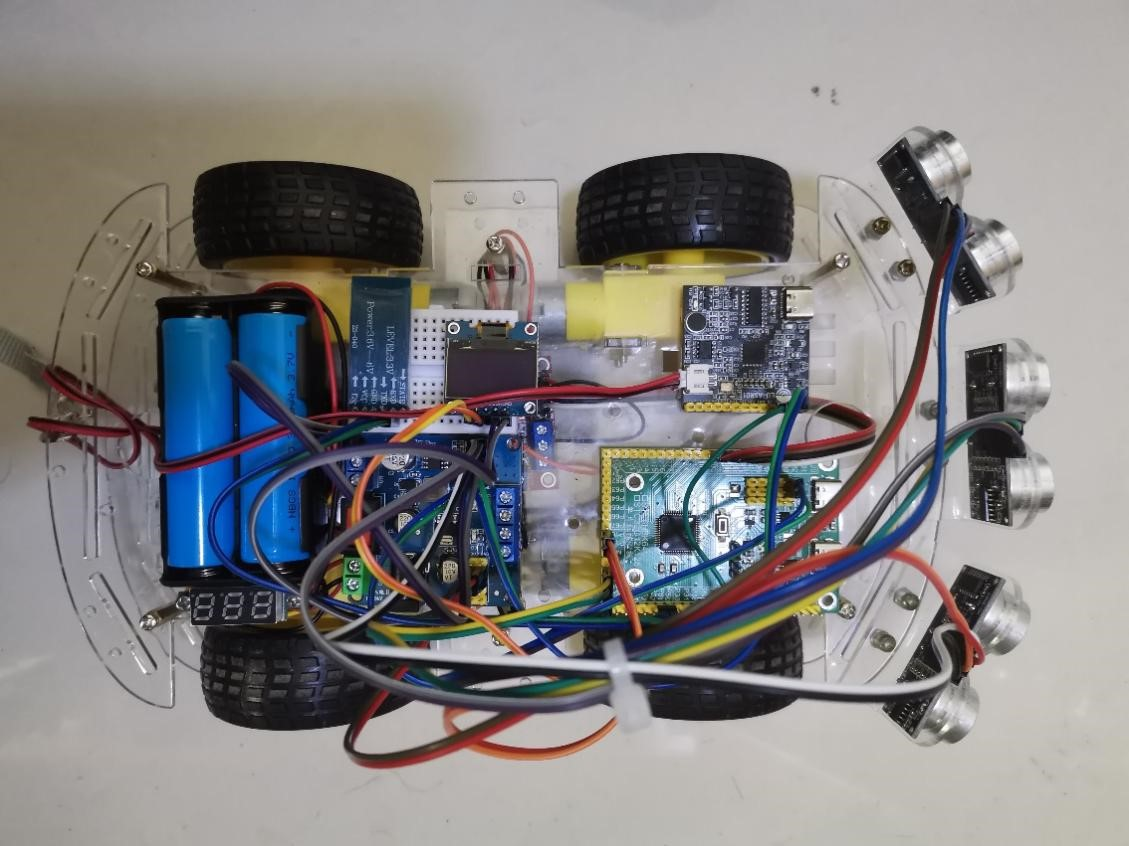
\includegraphics[width=0.5\textwidth]{figure/STC8H-CAR.jpg}
	\caption{基于STC8H的智能小车硬件实物图}
	\label{fig:app-stc8h-hardware}
\end{figure}

\subsubsection{功能与设计}

小车的核心逻辑围绕“模式切换”展开，共三种模式：

\begin{enumerate}
	\item 蓝牙遥控模式：手机或电脑通过蓝牙发送字符指令（'R'/'S'/'T'切换模式，'0'停止，'1'/'2'前进后退，'3'/'4'转向），单片机串口中断接收并执行。
	\item 循迹模式：五路TCRT5000L红外传感器检测黑线位置，输出信号组合决定小车转向方向（左偏则右转，右偏则左转，全在黑线上则直行）。
	\item 超声波避障模式：HC-SR04测距，距离小于阈值时自动转向避开障碍物。
\end{enumerate}

语音模块ASR-ONE通过串口发送指令，与蓝牙共用同一套模式切换逻辑。语音唤醒词为“糖果”，唤醒后可说出“遥控模式”“循迹模式”“避障模式”切换状态。

\subsubsection{代码结构}

项目代码共约800行C语言，核心结构如下：

\begin{itemize}
	\item 主循环：轮询蓝牙串口接收标志和超声波测距，主函数仅约20行；
	\item Motor.c：PWM调速（STC8H的PCA模块）、前进/后退/转向/停止函数；
	\item FollowLine.c：五路循迹传感器的读取与转向决策；
	\item Ultrasonic.c：超声波触发测距与距离计算；
	\item OLED.c：I2C驱动与汉字取模显示（显示项目名称和制作者信息）。
\end{itemize}

串口接收采用中断方式，UART3接收到数据后置标志位，主循环根据标志位执行对应动作。这和第~\ref{ch:scheduler-and-state-machine}~章“标志位法”的调度思想一脉相承——只是当时作者还没意识到这叫做“非阻塞编程”。

\subsubsection{成果与反思}

项目获得了省级奖项，但更重要的是让作者第一次完整经历了“需求分析 → 硬件选型 → 电路焊接 → 软件调试 → 联调测试”的全流程。几个关键教训如下：

\begin{enumerate}
	\item 语音模块在嘈杂环境下识别率下降明显，竞赛现场需要靠近麦克风才能唤醒；
	\item L298N模块发热严重，长时间运行后PWM输出不稳定，小车速度忽快忽慢；
	\item STC8H的RAM只有约8KB，不敢用任何动态内存分配，所有数组都静态定义——这也直接影响了作者后来对第~\ref{ch:memory-alloc}~章“静态内存池”的偏好。
\end{enumerate}

这个项目的代码风格还很稚嫩（所有逻辑堆在main.c里、几乎没有模块化），但它为作者后来的工程习惯奠定了基础：先跑通、再优化、交期优先。


\subsection{STC51温控系统（2024年）}

这是作者在大学课程设计期间完成的项目，硬件基于STC89C52RC单片机（51内核，主频11.0592MHz），核心功能是温度采集、显示、报警与步进电机控制。虽然硬件资源极度有限（RAM约512字节，Flash约64KB），但作者在这个项目里第一次尝试了“菜单框架”的设计，为第~\ref{ch:menu-system}~章的菜单系统提供了最初的灵感。

\subsubsection{技术栈}

\begin{itemize}
	\item 主控：STC89C52RC（经典51单片机）
	\item 温度传感器：DS18B20（单总线数字温度传感器）
	\item 显示：LCD12864（带中文字库，串行/并行可选）
	\item 存储：AT24C02（I2C EEPROM，用于保存参数）
	\item 时钟：DS1302（实时时钟芯片，带备用电池）
	\item 执行：步进电机（28BYJ-48，ULN2003驱动）、蜂鸣器
	\item 输入：4个独立按键
\end{itemize}

\subsubsection{菜单框架设计}

这是项目最核心的部分。LCD12864显示4行，每行可显示8个中文字符或16个英文字符。菜单系统要实现的功能包括：

\begin{enumerate}
	\item 主界面显示：年月日、时分秒、星期、温度（摄氏/华氏/模拟三种模式）；
	\item 子菜单：时间设置、闹钟设置、温度报警阈值设置、步进电机模式设置、历史温度查看；
	\item 参数编辑：选中参数高亮闪烁，按键加减调整，确认保存到EEPROM。
\end{enumerate}

代码结构分为三层：

\begin{itemize}
	\item UI.c：菜单框架核心，维护\texttt{ui\_range\_from}、\texttt{ui\_range\_to}、\texttt{ui\_selected}三个变量控制菜单滚动与选中；
	\item UI\_ClickEvent()：根据选中项分发到不同设置界面（时间/闹钟/温度/步进电机/历史记录）；
	\item 每个设置界面使用状态机管理编辑焦点（select\_set变量），闪烁显示当前正在编辑的字段。
\end{itemize}

菜单项定义为一个二维字符数组：

\begin{lstlisting}[style=c]
	uint8_t code UI_items[ITEM_COUNT][17] = {
		"时间设置",
		"闹钟设置",
		"报警温度设置",
		"步进电机设置",
		"历史温度查看"
	};
\end{lstlisting}

按键处理采用第~\ref{ch:scheduler-and-state-machine}~章介绍的“非阻塞轮询”方式——定时器中断每10ms扫描一次按键状态，主循环通过\texttt{Keys\_GetKey()}读取键值，菜单更新函数根据键值决定操作（进入/退出/上移/下移/确认）。

\subsubsection{EEPROM参数存储}

所有用户可调参数（温度单位模式、闹钟时间、报警阈值、步进电机阈值）都保存在AT24C02中。上电时通过\texttt{Read\_Init()}读取并恢复，修改后通过\texttt{AT\_WriteByte()}或\texttt{AT\_WriteBytes()}立即保存。这和正文第~\ref{ch:param-store}~章介绍的“魔数+结构体整包保存”思路一致——只是当时作者用的是逐字节保存，因为没有定义统一的结构体布局。

\subsubsection{步进电机联动}

步进电机根据温度与阈值的比较结果自动正转或反转：

\begin{itemize}
	\item 模式1（真实温度）：温度高于StepMotorHigh\_C时正转，低于StepMotorLow\_C时反转；
	\item 模式2（模拟温度）：同上，但使用模拟温度值（用于演示，无需传感器）。
\end{itemize}

步进电机驱动在定时器中断中调用\texttt{StepMotor\_Run()}，通过相序数组控制四相绕组依次通电，实现精确的步进角度控制。

\begin{table}[htbp]
	\centering
	\caption{温控系统与正文各章的对应关系}
	\label{tab:app-temp-mapping}
	\begin{tabular}{lll}
		\toprule
		正文章节 & 对应功能 & 项目中的实现 \\
		\midrule
		第~\ref{ch:scheduler-and-state-machine}~章 & 非阻塞调度 & 定时器中断 + 主循环轮询 \\
		第~\ref{ch:menu-system}~章 & 菜单框架 & UI.c中的滚动选择与状态编辑 \\
		第~\ref{ch:param-store}~章 & 参数存储 & AT24C02保存用户配置 \\
		第~\ref{ch:memory-alloc}~章 & 静态内存 & 全部静态分配，无malloc \\
		\bottomrule
	\end{tabular}
\end{table}


\subsection{“挑战杯”RK3588智能车（2025年，未完成）}

这是作者唯一一个“画了饼但没有跑通”的项目，项目的初衷是“用国产RK3588芯片替代NVIDIA Jetson做SLAM导航”，实现从底层控制到上层视觉的完整系统。

\subsubsection{设计目标}

\begin{itemize}
	\item 主控：STM32F407VET6（运动控制）+ 香橙派5MAX（RK3588，8GB内存，6TOPS NPU）
	\item 感知：YDLIDAR X3激光雷达（三角测距，360度扫描）、MPU6050/JY901B陀螺仪
	\item 底盘：麦克纳姆轮四驱（全向移动）
	\item 软件：ROS2 + SLAM建图导航 + AI路径规划
	\item 显示：2.4寸TFT LCD
\end{itemize}

\begin{figure}[htbp]
	\centering
	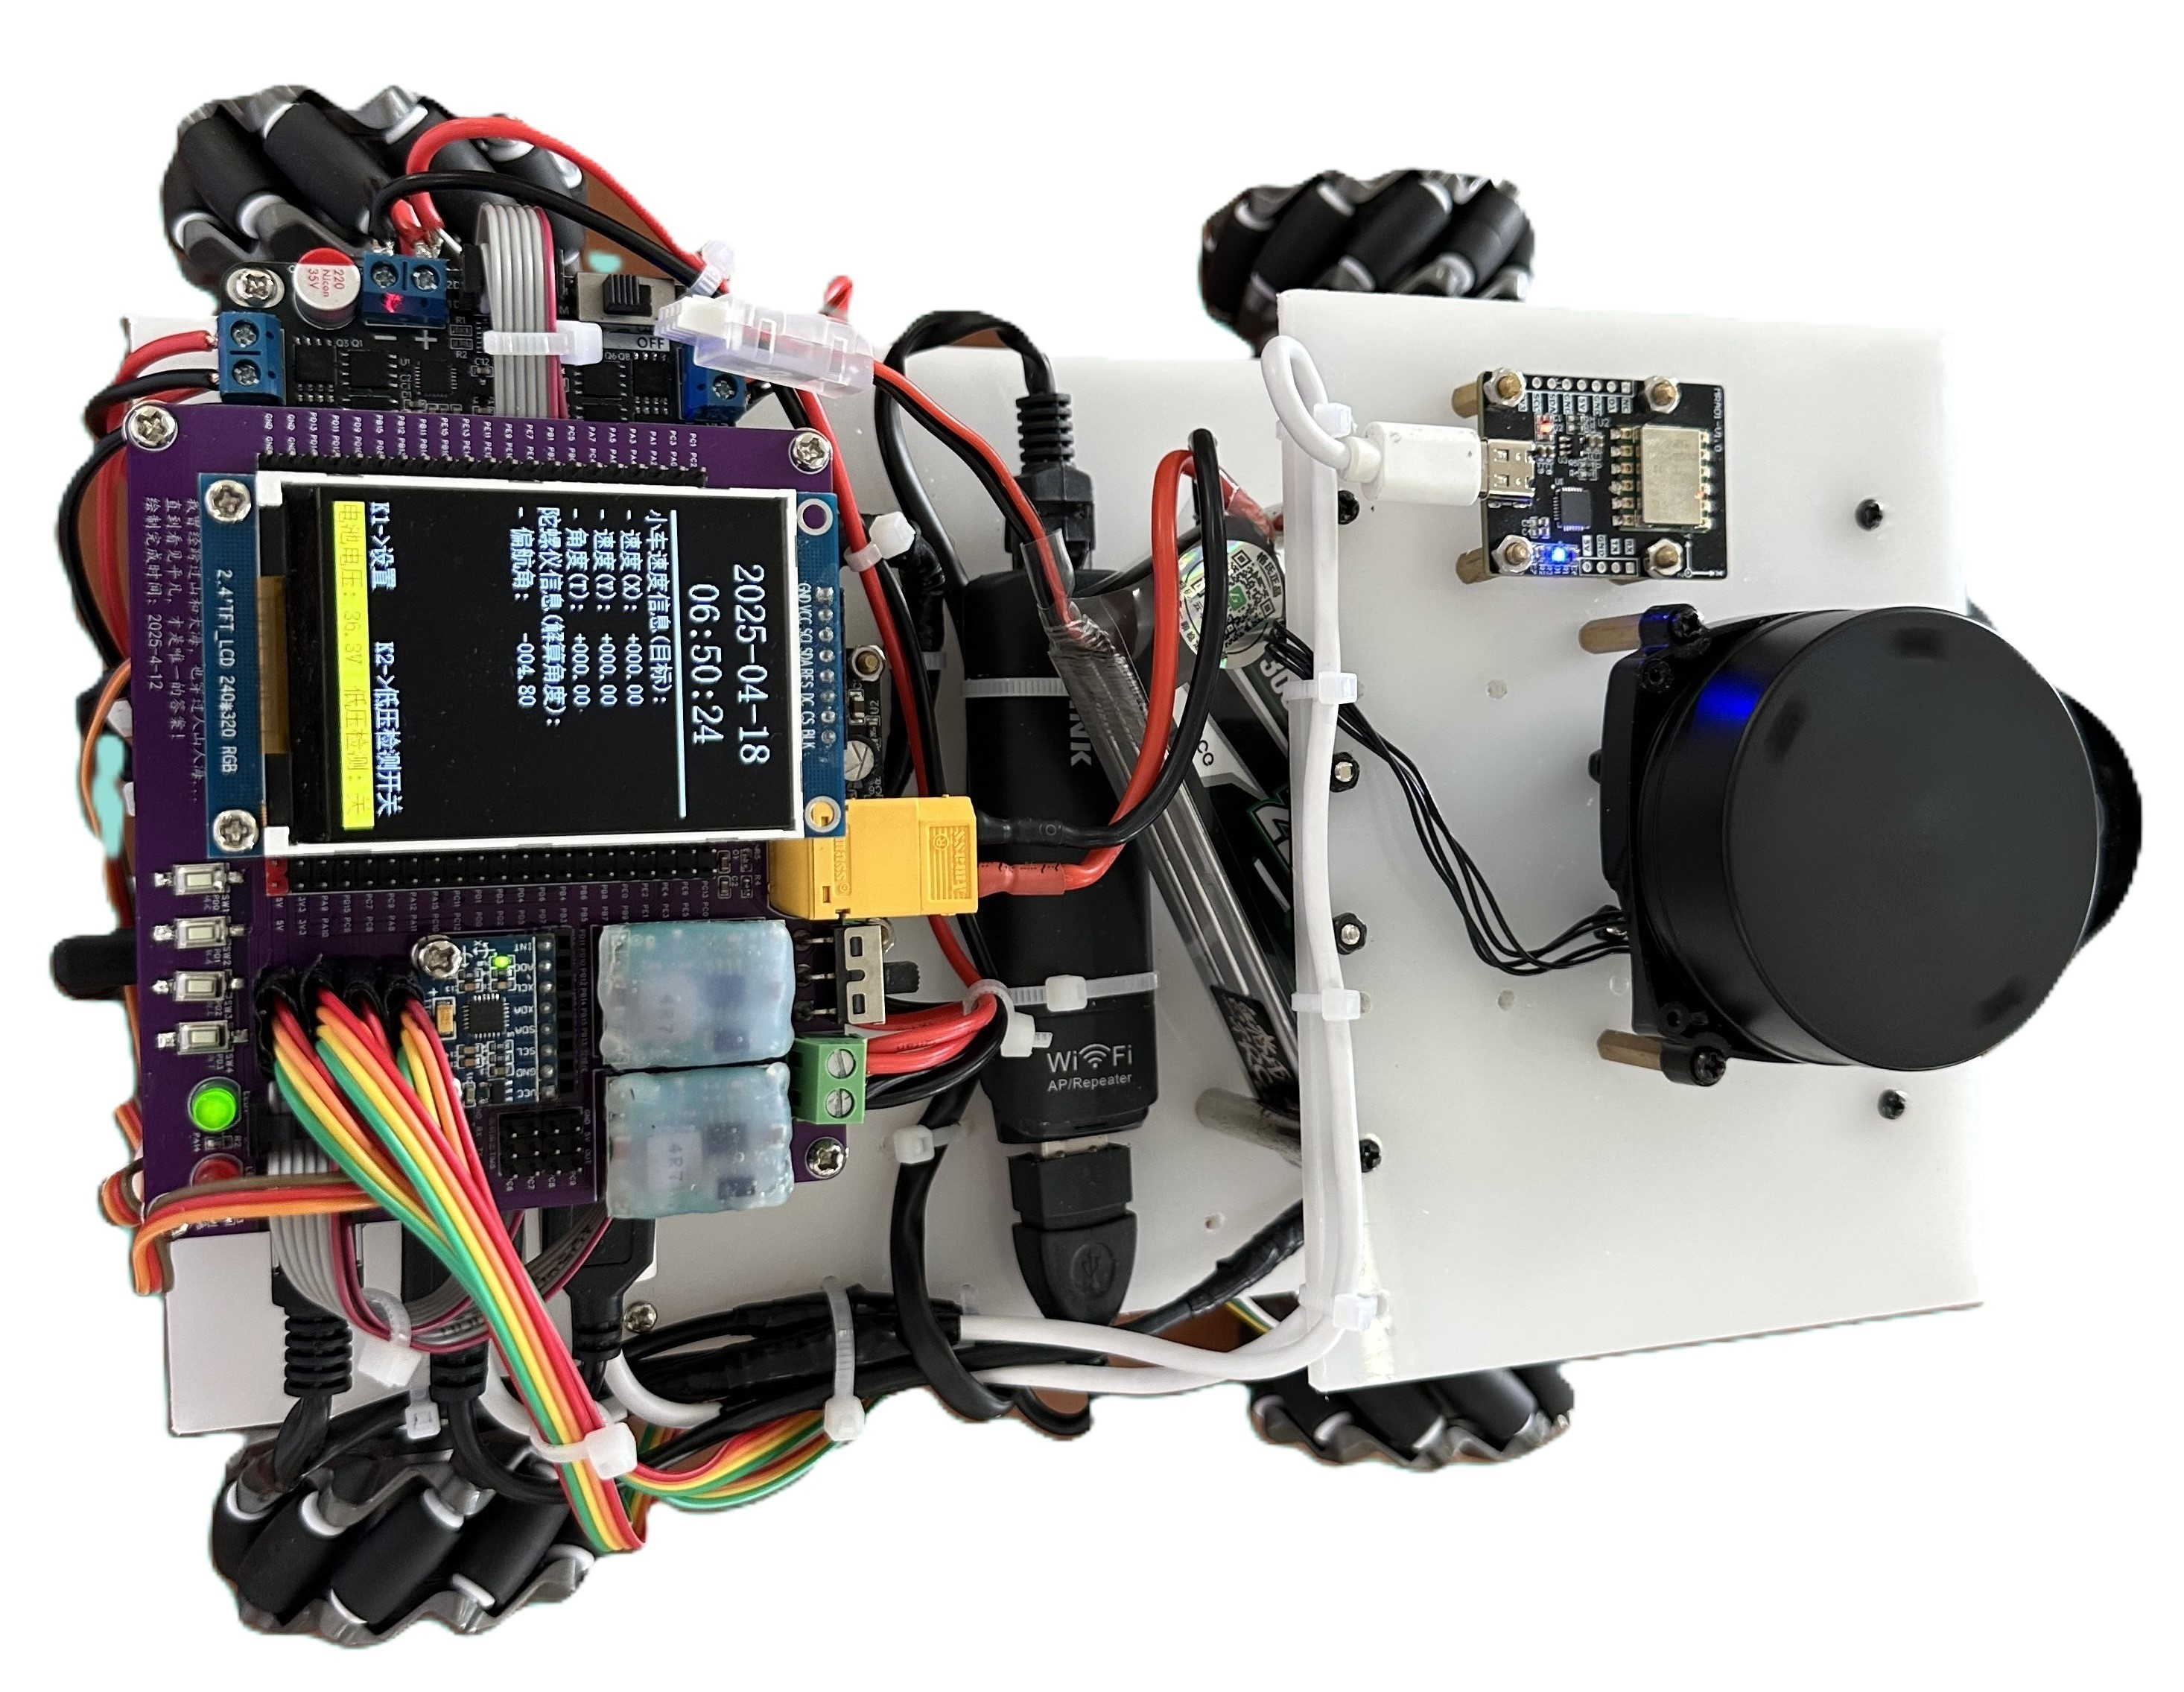
\includegraphics[width=0.5\textwidth]{figure/RK3588-CAR.jpg}
	\caption{RK3588智能车硬件组装图}
	\label{fig:app-rk3588-hardware}
\end{figure}

\subsubsection{为什么没有完成}

项目在硬件层面进展顺利——STM32F407的电机PID控制、串口通信、陀螺仪姿态解算都调通了，激光雷达也能正常输出点云数据。但到了RK3588端的软件集成阶段，项目彻底卡住了。

根本原因只有一个：香橙派是一个“封闭的平台”。

开发者拿到的不是一套可深入的系统，而是一个“黑盒”——官方提供了镜像文件、几个编译好的二进制工具、以及一份超过1000页的PDF文档。但仔细翻看就会发现，这1000页里翻来覆去讲的是同一件事：怎么用镜像烧录工具把系统装进SD卡、怎么用HDMI接显示器看桌面、怎么运行官方预置的几个测试程序（比如NPU推理demo、摄像头采集demo）。至于“系统为什么这样配置”、“驱动是怎么工作的”、“遇到编译错误怎么排查”、“如何把第三方库移植进来”——一个字都没有。

具体到ROS2集成时，问题变成了这样：

\begin{enumerate}
	\item 官方的Ubuntu镜像为了“稳定”，裁剪了大量开发库。安装ROS2需要的依赖时，\texttt{apt}频繁报错说“缺少依赖包”，但这些包的名称在香橙派的镜像源里根本找不到——因为官方源只维护了最基本的系统组件，不维护ROS2相关的包。作者不得不手动从源码编译这些依赖，但编译过程中又发现系统头文件缺失、库版本不匹配、ABI不一致；
	\item 官方提供的NPU推理demo能跑通，但那是“演示级”的代码——它只是告诉你“NPU可以工作”，但没有提供任何关于“如何将自定义模型转换为RKNN格式”的完整文档。作者按照官方文档转换YOLO模型时，转换工具频繁报出“不支持的操作符”错误，而官方论坛上关于这个问题的回复只有一句“请检查模型格式”——然后就没有然后了；
	\item 那份1000页的文档，在作者遇到具体问题时几乎派不上用场。它告诉了你“怎么用”，却没有告诉你“为什么这样用”和“遇到问题怎么办”。作者在论坛上翻到的同类问题，最早的提问时间是一年前，至今没有官方回复。
\end{enumerate}

这个项目最终止步于“能跑但跑不稳”的状态：激光雷达能建图，但地图质量差；电机能控制，但SLAM的定位精度不够；STM32和RK3588能通信，但ROS2节点经常异常退出。作者在截止日期前提交了项目书，但实物演示未能达到预期效果。

这次失败让作者深刻认识到：在嵌入式开发中，“开发板的性能参数”和“开发板的可用性”是两回事。一块开发板的价值，不只取决于它的CPU主频、NPU算力、内存大小，更取决于厂商为开发者提供了多少“可用的信息”——是否开放原理图、是否有完整的驱动源码、是否提供可移植的SDK、是否有活跃的社区和及时的官方支持。如果这些都没有，即便参数再好看，它也只是一块“昂贵的砖头”。

这也是后来毕业设计选择MaixCAM的重要原因之一——MaixCAM的算力只有1TOPS，远不如RK3588的6TOPS，但它的文档是公开的、源码是可读的、社区是活跃的。一个“性能弱但开放”的平台，在交期面前比“性能强但封闭”的平台更可靠。

\subsection{Java 成绩管理系统（2025 年）}

这是作者在大三下学期完成的一组课程设计作品，完成于 2025 年 4 月 5 日。当时同时修了《Java 项目实训》和《Java 热门框架》两门必修课，两门课都要求提交完整的 Web 课程设计，项目内容完全不同。

《Java 项目实训》要求开发一个物流管理系统。这类传统 JSP 框架的项目特点是“能跑，但极其难改”——页面逻辑写在 JSP 里，数据访问层与视图层严重耦合，每新增一个功能模块就要复制粘贴大量重复代码。作者花了一周时间完成这个系统，在开发过程中把数据模型加载、页面组件渲染和功能权限控制三个核心模块从具体业务中剥离出来，形成了一套可复用的框架底座。

随后在《Java 热门框架》课程中，作者需要开发一个学生信息管理系统。他没有从零开始，而是直接将上一项目中抽离出的框架底座套用过来，只需编写新的实体类和页面组装逻辑，就快速完成了第二个功能完整且不重复的系统。

\subsubsection{物流管理系统：开发内容（一周完成）}

物流管理系统采用传统 JSP 框架开发，作者在一周内完成了系统所有功能模块，同时在开发过程中做了以下抽象：

\begin{enumerate}
	\item 模型层抽象：引入 \texttt{@ModelClass} 和 \texttt{@ModelField} 注解，将数据库映射直接写在实体类字段上。\texttt{@ModelField} 的 \texttt{column} 属性被设为必填项，要求显式声明数据库列名，不依赖“驼峰转下划线”的自动推断。
	
	\item 视图层抽象：基于组合模式设计 \texttt{HtmlAtom}、\texttt{HtmlSet}、\texttt{HtmlSingle} 等组件类，将 HTML 页面拆解为可复用的组件树，最终递归渲染为完整页面，替代传统 JSP 中的脚本拼接。
	
	\item 权限层抽象：引入功能码映射表，将“功能 ID → 允许访问的角色列表”集中管理，替代散落在各处的 if-else 判断。
\end{enumerate}

\subsubsection{框架底座：从物流管理系统中剥离}

物流管理系统完成后，作者发现上述三个模块与“物流管理”这个具体业务没有任何绑定关系——它们只依赖实体类上的注解、一个统一的页面渲染接口和一张权限映射表。于是把这三个模块抽成一套独立的框架代码，打包后可以直接导入其他项目使用。

\subsubsection{学生信息管理系统：框架底座的应用}

在《Java 热门框架》课程中，作者直接导入了上一步抽离出的框架底座，只需要做三件事：编写新的实体类（学生、课程、成绩等）并添加注解、组装已有的 HTML 组件形成新页面、配置新的功能码与角色映射关系。整个学生信息管理系统的开发时间大幅缩短，且代码量比从头写减少了约 60\%。

\begin{table}[htbp]
	\centering
	\caption{两个课程设计与正文的对应关系}
	\label{tab:app-java-mapping}
	\begin{tabular}{lll}
		\toprule
		正文章节 & 对应思想 & 本项目中的体现 \\
		\midrule
		第~\ref{ch:script-engine}~章 & 生成器思想 & 注解驱动生成 SQL 与 HTML \\
		第~\ref{ch:command-parser}~章 & 表驱动分发 & 功能码 + 角色映射表控制权限 \\
		第~\ref{ch:menu-system}~章 & 组合模式 UI & HtmlAtom 组件化视图渲染 \\
		\bottomrule
	\end{tabular}
\end{table}

\subsubsection{小结}

这次课程设计的核心不是“写了两个管理系统”，而是：第一个项目用了一周时间完成物流管理系统，在开发过程中抽象出一套可复用的框架底座；第二个项目直接复用底座完成学生信息管理系统，省去了重复劳动。这和本书反复提到的“塑料轮子”逻辑一致——第一次造轮子是为了让项目跑起来，第二次把轮子拆下来装到新车上，是为了不再造第二个轮子。两门必修课最终都顺利通过了验收，而“一次搭建、两次复用”的经历，也让作者在后来设计 MetroEditor 的嵌入式导出模块时，更倾向于思考“哪些东西可以抽成通用骨架”，而不是每次都重新搭一遍地基。

\subsection{基于STM32H743与MaixCAM的双核异构智能小车（2026年）}

这是作者本科阶段最重要的项目，也是本书正文中反复引用的案例。项目的核心决策是：放弃ROS2，用“塑料轮子”方案在交期内交付一个可演示的系统。

\subsubsection{硬件架构}

\begin{itemize}
	\item 主控1：STM32H743XIH6（Cortex-M7，480MHz，1MB RAM，2MB Flash），负责运动控制、传感器融合与底层决策；
	\item 主控2：MaixCAM边缘视觉模块（RISC-V双核，1TOPS NPU），负责YOLOv5s路标识别；
	\item 通信：高速串口（921600bps），自定义HEX帧协议（见第~\ref{ch:serial-fifo}~章）；
	\item 传感器：ICM42688六轴陀螺仪（姿态解算）、镭神N10P激光雷达（TOF，12m测距）、HC-SR04超声波（前后各一）、520霍尔编码器电机（四轮）；
	\item 执行：逐飞科技DRV8701有刷电机驱动模块（×2）、舵机云台（双轴）；
	\item 显示：2.0寸TFT-LCD（240×320，ST7789V2驱动）；
	\item 电源：3S锂电池（11.1V）经TPS5430、RT9013、MP1584多路稳压。
\end{itemize}

\begin{figure}[htbp]
	\centering
	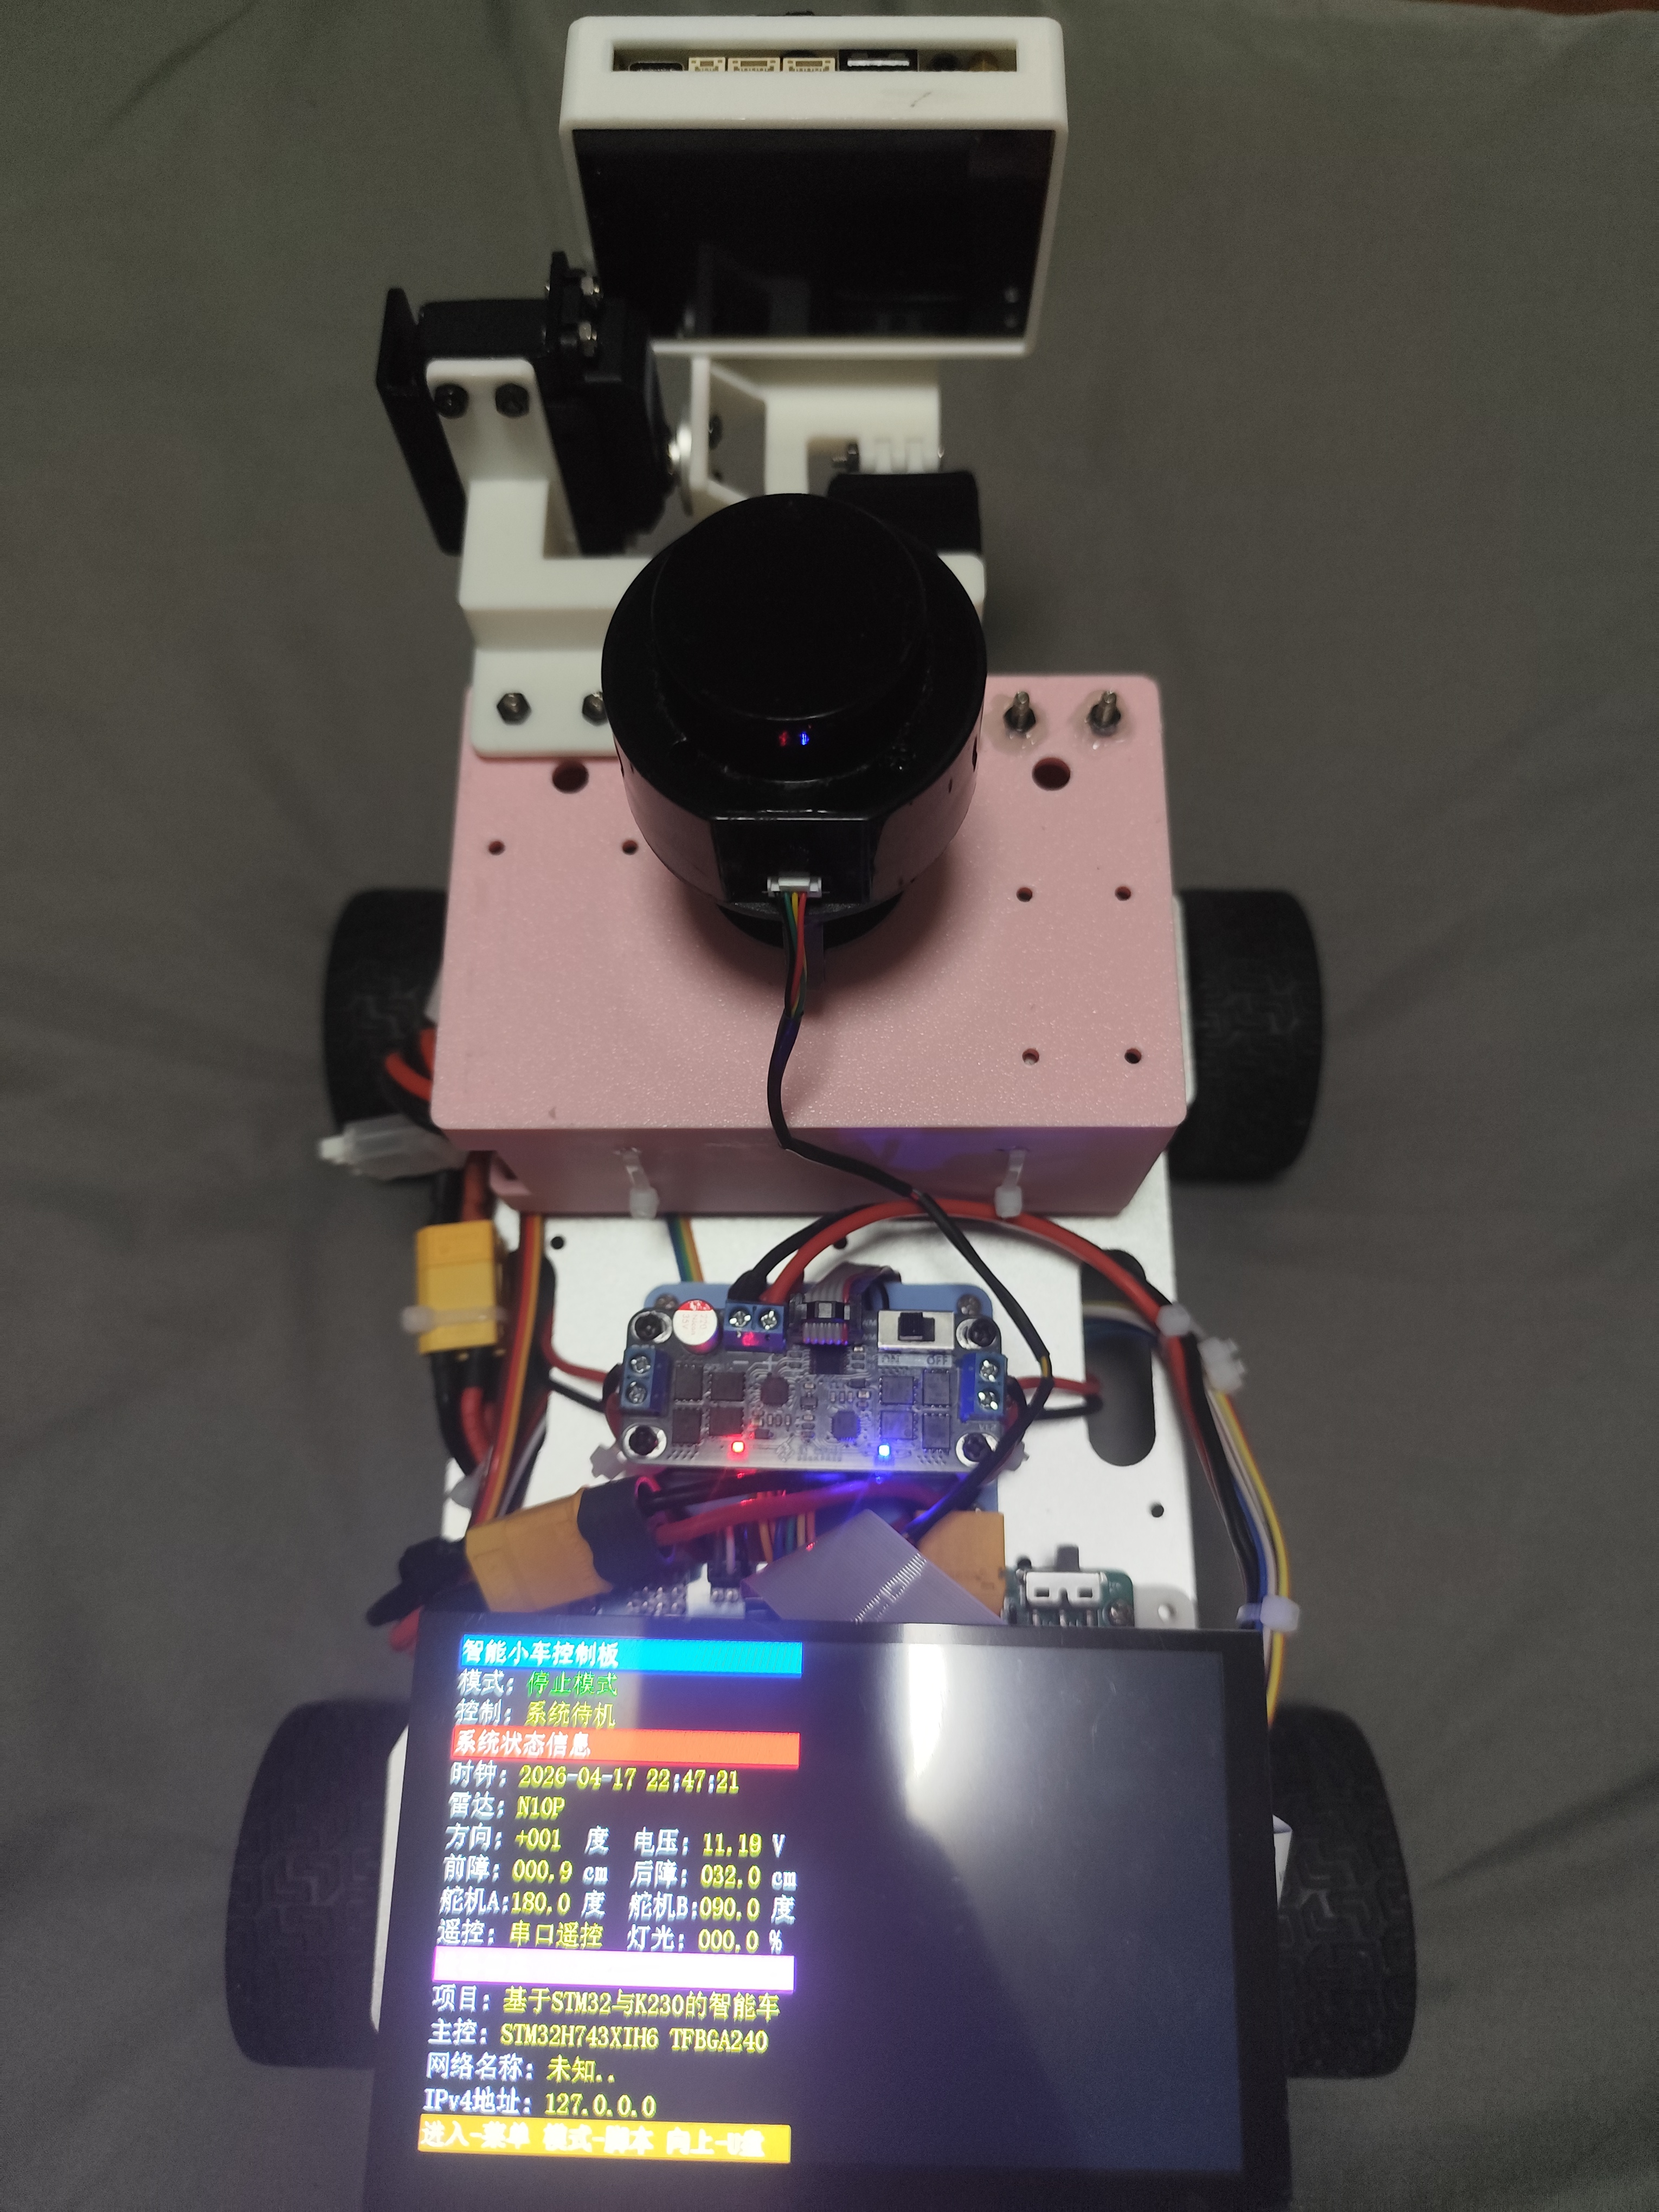
\includegraphics[width=0.5\textwidth]{figure/K230-CAR.jpg}
	\caption{毕业设计智能小车硬件实物图}
	\label{fig:app-graduation-hardware}
\end{figure}

\subsubsection{STM32端软件架构}

系统不依赖RTOS，采用第~\ref{ch:simple-task}~章介绍的\texttt{simple\_task}轻量级协作式调度器。TIM6提供1ms系统节拍，主循环通过\texttt{Task\_Loop()}调度就绪任务；TIM7中断中执行\texttt{Car\_Tick()}，完成电机PID控制等硬实时任务（控制周期1ms）。

主要任务划分如下：

\begin{table}[htbp]
	\centering
	\caption{毕业设计STM32端任务划分}
	\label{tab:app-graduation-tasks}
	\begin{tabular}{lll}
		\toprule
		任务名 & 周期 & 功能 \\
		\midrule
		Main\_Task & 50ms & 系统监控（电池电压、RTC、待机策略） \\
		IMU\_Task & 10ms & ICM42688数据解析、Mahony互补滤波姿态解算、里程计融合 \\
		Lidar\_Task & 100ms & N10P激光雷达数据读取与避障决策 \\
		NRF24L01\_Task & 100ms & 遥控器数据接收与体感指令生成 \\
		Condition\_Task & 100ms & 条件域表达式评估与响应触发 \\
		CS200A\_Task & 20ms & 超声波测距触发、中值滤波 \\
		GUI\_Task & 200ms & TFT-LCD显示（模式、速度、坐标、电池电量）与菜单交互 \\
		Car\_Tick（硬实时） & 1ms & PID控制、编码器读取、电机PWM输出（TIM7中断） \\
		\bottomrule
	\end{tabular}
\end{table}

\subsubsection{自适应里程计融合算法}

这是项目的一个核心创新点，正文第~\ref{ch:about-author}~章有提及，这里补充技术细节。

轮式机器人的里程计在轮胎打滑时会失效——编码器转了很多圈，但小车并没有移动相应距离。传统的EKF（扩展卡尔曼滤波）可以融合IMU和编码器，但其性能依赖精确的系统模型，且需要实时计算雅可比矩阵，在嵌入式平台上计算负载较高。

作者提出的替代方案是：定义“打滑度检测函数”\(P(x,y)\)，根据PID输出量与编码器实测值的比值关系判断打滑程度，然后通过线性加权动态调整编码器和IMU的融合权重。

关键公式如下：

\begin{equation}
	\alpha = \max_{i \in A} P\left(100 \times \frac{v_{i,O}(t_i)}{v_{i,A}(t_i)},\ 100 \times \frac{v_{i,O}(t_{i-1})}{v_{i,A}(t_{i-1})}\right)
\end{equation}

其中\(v_{i,O}\)是PID输出量（期望速度），\(v_{i,A}\)是编码器实测速度。当打滑严重时，\(\alpha\)趋近于1，系统更信任IMU里程计；当打滑轻微时，\(\alpha\)趋近于0，系统更信任编码器里程计。

最终融合公式为：

\begin{equation}
	v_{\text{DOM}}(k+1) = (1-\gamma) \cdot v_{\text{ENC}}(k) + \gamma \cdot v_{\text{IMU}}(k)
\end{equation}

其中\(\gamma = \min\{k_1 \alpha + k_2 \beta + \theta, 1\}\)，\(\beta\)是前后轮间的打滑度，\(\theta\)是固定转换阈值。

测试结果表明，该算法的里程计相对误差最大0.97\%，平均0.46\%，标准差0.24\%，优于纯编码器方案在打滑路面上的表现。

\subsubsection{MaixCAM端视觉推理}

MaixCAM运行MicroPython，通过MaixPy的NN库加载YOLOv5s量化模型（.mud格式）。推理流程如下：

\begin{enumerate}
	\item GC2093摄像头采集图像（640×480），预处理（padding + resize至320×320）；
	\item NPU推理，输出检测框（含坐标、置信度、类别ID）；
	\item 根据类别ID查表（send\_commands字典），通过串口发送对应的条件域指令；
	\item 同时绘制检测框并显示于显示屏。
\end{enumerate}

YOLOv5s模型在自定义路标测试集上的mAP50达到0.995，推理帧率约15FPS，满足实时性要求。

\subsubsection{条件域指令协同机制}

这是STM32与MaixCAM之间“智能协同”的核心——视觉识别结果不是简单地触发固定动作，而是通过条件域指令实现动态决策。

条件域指令格式：

\begin{lstlisting}
	cond set <条件ID> "<表达式>" "<响应动作>" [销毁时间（秒）]
\end{lstlisting}

示例：当检测到类别ID为p14（禁止停车标志）时，发送指令：

\begin{lstlisting}
	cond set 1 "dx>0.2 & abs(dy)<0.5" "t_dyaw:=100-dw" 30
\end{lstlisting}

STM32端解析该指令后，会在30秒内持续监测局部坐标系下的位置增量（dx、dy）和偏航角增量（dw）。当条件满足时，自动执行响应动作（此处为转向修正）。若超时未满足条件，则触发声光报警。

这个机制让系统从“收到指令就执行”升级为“根据实时状态判断是否执行”，是正文第~\ref{ch:script-engine}~章表达式解析器的最直接应用。

\subsubsection{裸机阶段的“四面出击”与失败教训}

在调度器从裸机切换到FreeRTOS之前，作者在裸机框架下尝试过三个“高级功能”——ROS2集成、Lua脚本引擎、RDK X5视觉部署。这三个方向最终都未能成为交付方案的核心，但它们的失败本身构成了毕业设计最重要的经验来源。毕业论文第5.5.4节（ROS2测试）和第5.5.5节（Lua脚本运行）正是这些尝试的历史残留。

\textbf{第一次尝试：ROS2集成（2025年7月—9月）}

作者尝试将小车接入ROS2系统。当时的设想是：STM32作为底层运动控制节点，通过串口与运行ROS2的Linux开发板通信；上位机运行导航、建图等高级功能。硬件选型是香橙派5MAX（RK3588，8GB内存），运行Ubuntu 22.04 + ROS2 Humble。

具体工作包括：在RK3588上编译ROS2的串口通信包（serial）、编写ROS2节点（C++）订阅/cmd\_vel话题将速度指令下发至STM32、STM32端新增ROS2命令解析分支。

三个月的尝试后，项目卡在了以下问题上：ROS2的serial包在ARM架构下编译依赖复杂，串口数据帧偶尔出现粘包和丢包；RK3588的NPU工具链（RKNN）对YOLO模型的支持不完善；ROS2节点启动顺序难以控制（STM32上电即运行，但RK3588需约30秒初始化）。到2025年9月底，作者决定暂时搁置ROS2方向。

\textbf{第二次尝试：Lua脚本引擎移植（2025年10月—11月）}

作者尝试在STM32上移植Lua解释器，目标是让用户可以通过SD卡加载Lua脚本，实现“无需重新编译即可改变小车行为”的可编程能力。

具体工作包括：将eLua移植到STM32H743上（适配静态内存池）、导出C API（Car\_Control、IMU\_GetEuler等注册为Lua模块）、实现SD卡脚本加载功能。

移植工作本身是成功的——Lua解释器能在STM32上运行，示例脚本（小车前进.lua、陀螺仪数据显示.lua）都能正常执行。但Lua解释器占用约40KB Flash和8KB RAM；实时控制任务无法使用解释型语言；用户实际需要的“参数调整”和“行为配置”已被字符串命令系统和FatFS覆盖。最终Lua引擎作为“技术验证”保留在代码仓库中，但默认不编译进交付固件。

\textbf{第三次尝试：RDK X5视觉部署（2026年1月—2月）}

作者尝试将视觉推理从MaixCAM迁移到RDK X5（基于RK3588系，6TOPS算力）。理论上RDK X5能运行更大更精确的模型。

测试结果：YOLOv5n（18ms，mAP50=0.82）、YOLOv5s（35ms，mAP50=0.89）、YOLOv5m（72ms，mAP50=0.91）。

虽然推理速度比MaixCAM更快，但端到端延迟并未显著降低（RDK X5的串口通信栈更复杂）；RDK X5功耗远高于MaixCAM（约5W vs 1.5W）；最关键的是，距离答辩只剩两个月，切换平台的时间成本已超出预算。最终MaixCAM方案被保留为交付方案的核心。

这三个失败的共同点是：作者在项目早期低估了“把一个新技术集成到现有系统中”的边际成本——不仅要让新技术本身跑起来，还要保证它与现有系统的接口稳定、资源不冲突、调试可追踪、维护可持续。

\subsubsection{调度器选型：从裸机到FreeRTOS再到simple\_task}

毕业设计的软件架构经历过一条完整的时间线：裸机（2025年7月—2026年2月）→ FreeRTOS（2026年3月—4月）→ simple\_task（2026年6月）。这不是简单的工具替换，而是一场持续近一年的技术认知升级。

\textbf{第一阶段：裸机（2025年7月—2026年2月）}

项目最初的代码是典型的裸机轮询：一个巨大的\texttt{while(1)}循环里依次调用\texttt{IMU\_Tick()}、\texttt{Car\_Tick()}、\texttt{Key\_Tick()}、\texttt{UI\_Update()}、\texttt{Lidar\_Tick()}，中间穿插着若干个\texttt{Delay\_ms()}。这种写法在项目初期只有三五个功能时还能应付，但到了2025年底，随着激光雷达、超声波、NRF24L01遥控、条件域解析器、GUI菜单、串口命令系统等十多个功能陆续加入，主循环已经臃肿到难以维护的程度。

裸机阶段暴露了三个核心问题：主循环轮询导致周期控制失效（IMU解算需要稳定的10ms周期，但一旦LCD刷新等耗时任务跑久，后续任务都会被推迟）；\texttt{Delay\_ms()}阻塞主循环（有效任务执行时间占比不到30\%）；代码维护困难（一个main.c文件2000多行，改一处可能破坏三个不相关的功能）。

\textbf{第二阶段：FreeRTOS（2026年3月—4月）}

2026年3月初，作者引入了FreeRTOS。拆分的理由非常充分：每个功能模块变成独立任务，通过信号量和队列通信，抢占式调度保证高优先级任务不被低优先级任务拖累。答辩前的两个月里，作者把IMU解算、运动控制、按键扫描、UI刷新、串口解析分别拆成了\texttt{vTask}，并成功让小车跑了起来。

FreeRTOS阶段解决了一些问题：10ms的IMU任务不再被其他任务干扰；任务隔离让代码结构清晰了不少；答辩PPT上可以写“基于FreeRTOS的实时多任务系统”。

但问题也随之出现：任务栈大小难以精确估算（栈溢出的后果是随机HardFault）；抢占式调度引入了新的不确定性（串口FIFO的临界区保护变得更复杂）；FreeRTOS在这个项目里只用了约20\%的功能（任务调度+信号量），却承担了100\%的复杂度和风险。

2026年4月答辩顺利通过。但作者心里清楚，答辩PPT上的FreeRTOS架构图和实际调试中遇到的信号量死锁、栈溢出、任务优先级反转，是两回事。

\textbf{第三阶段：simple\_task（2026年6月，后续复盘）}

答辩结束后，作者重新审视了项目的调度需求：所有任务的执行时间都是微秒级别；任务之间不需要抢占，只需要协作式轮转；周期控制可以用定时器中断统一管理。

于是作者花了半天时间，写了一个只有二百多行的轻量级调度器，后来被正式命名为\texttt{simple\_task}。它的核心逻辑极其简单——定时器中断累加每个任务的\texttt{tickCount}，主循环遍历任务池、执行所有到期任务。任务状态只有四个：WAIT、READY、RUN、DISABLE，状态转换是线性的，没有任何抢占和优先级。

\begin{lstlisting}[style=c]
	/* 简化版 simple_task 核心逻辑 */
	void Task_Tick(void)              /* 1ms 定时器中断调用 */
	{
		for (i = 0; i < TASK_MAX_COUNT; i++) {
			if (task[i].state == WAIT) {
				task[i].tickCount++;
				if (task[i].tickCount >= task[i].period) {
					task[i].state = READY;
				}
			}
		}
	}
	
	void Task_Loop(void)              /* 主循环中调用 */
	{
		for (i = 0; i < TASK_MAX_COUNT; i++) {
			if (task[i].state == READY) {
				task[i].callback();
				task[i].state = WAIT;
				task[i].tickCount = 0;
			}
		}
	}
\end{lstlisting}

这个二百多行的调度器恰好满足了项目的全部需求：任务数量固定、静态分配、不依赖malloc；每行代码都能看懂，单步跟踪时不会跳进黑盒；RAM占用比FreeRTOS方案少了约4KB，Flash少了约15KB；CPU利用率从裸机时期的不足30\%提升到了80\%以上。

有趣的是，\texttt{simple\_task}的雏形早在2026年2月就已经存在——作者当时为了调试某段代码写过一个小型的任务轮询器，但没有正式命名。真正让它成为“调度器”并写进仓库，是答辩后的这次复盘。

一个诚实的注脚：毕业答辩的论文里还保留着FreeRTOS的痕迹，因为那是2026年4月答辩前定稿的。值得说明的是，RTOS 方案仅用于前期的交期验证与流程评审；实际交付的代码库已于 6 月完成迁移，底层调度器切换为第 3 章介绍的 \texttt{simple\_task} 协作式任务调度器。这一调整使系统在保持原有功能完整性的前提下，显著降低了 RAM/ROM 占用，同时消除了抢占式调度带来的执行时序不确定性，提升了长期维护的可靠性。

\subsubsection{成果}

演示视频按时交付，论文答辩顺利通过。系统实现了：

\begin{itemize}
	\item 遥控模式（体感遥控 + NRF24L01无线控制）
	\item 自动避障（激光雷达点云分区 + 超声波辅助）
	\item 航向锁定（Mahony互补滤波姿态解算）
	\item 路标识别触发安全策略（条件域指令）
	\item 里程计定位误差小于2\%
\end{itemize}


\section{职场与业余项目：从功能到产品}


\subsection{SleepReminder——“电子监狱”（2026年）}

这是一个纯软件项目，但它的故事比很多硬件项目更曲折。SleepReminder是一个全屏强制提醒工具，旨在帮助作者自己克服熬夜写代码的习惯。项目的开发过程本身就是一个“与自己较劲”的寓言——作者写了一篇短篇小说《我把自己关进了亲手造的电子监狱》（\texttt{story.pdf}）记录这段经历。

\begin{figure}[htbp]
	\centering
	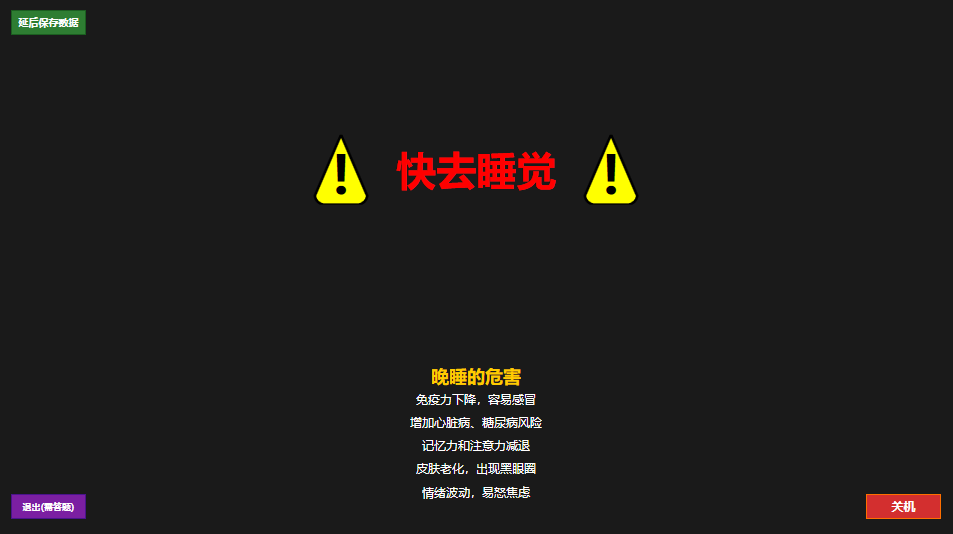
\includegraphics[width=0.8\textwidth]{figure/SleepRemider.png}
	\caption{SleepReminder界面设计图}
	\label{fig:sleep-remider}
\end{figure}

\subsubsection{技术栈}

\begin{itemize}
	\item 语言：C\#（WPF，.NET Framework 4.6.2）
	\item 系统交互：Windows API（进程管理、窗口枚举、注册表操作）
	\item 自启动：启动文件夹快捷方式（COM IWshRuntimeLibrary）
\end{itemize}

\subsubsection{功能迭代}

项目经历了六个版本的演进：

\begin{enumerate}
	\item V1.0（简单弹窗）：每天23:30弹窗，10分钟后锁屏。作者随手点“稍后”，继续写代码到凌晨。
	\item V2.0（反任务管理器）：用\texttt{EnumWindows}遍历窗口，发现任务管理器就\texttt{PostMessage}退出。作者用\texttt{taskkill /f /im}解决。
	\item V3.0（锁系统工具）：禁用CMD、PowerShell，改注册表。作者因为“好麻烦”而放弃抵抗——第一次“被自己的懒惰拯救”。
	\item V4.0（守护进程）：用C语言写守护进程，每秒检查主程序是否存活，被杀后立即重启。作者花了一个半小时跟自己的守护进程打攻防战，没写一行业务代码。
	\item V5.0（系统服务 + 三层嵌套）：注册为Windows系统服务，三层自我修复（主程序被杀→服务重启→被杀→重启计算机→再被杀→再重启）。CPU占用飙到70\%，作者拔了电源线。
	\item V6.0（BIOS方案，文学夸张）：故事中作者拆了笔记本电脑，热风枪吹下BIOS芯片，在ACPI表中嵌入定时关机逻辑。实际上并未真的焊主板，这个方案的真正意义是让作者意识到“战胜自己太麻烦”才是最终的解决方案。
\end{enumerate}

\subsubsection{与正文的对应关系}

这个故事虽然不涉及嵌入式代码，但它完美诠释了正文第~\ref{ch:deadline-ai}~章的观点——“AI是体力劳工，不是脑力军师”。作者在与自己搏斗的过程中，始终是“决策者”，代码只是执行者。那三层嵌套的守护进程不会自己决定“要不要重启”，它只会忠实地执行作者的意志——而作者需要对抗的，恰恰是自己的意志。


\subsection{地铁线路编辑器 MetroEditor（2026年）}

这是作者毕业后做的第一个完整工程工具项目，也是将毕业设计中积累的系统设计能力迁移到纯软件领域的尝试。MetroEditor是一个地铁线路数据编辑、编译、可视化与分析工具，配套Android客户端实现地图推送与记录同步。

\subsubsection{技术栈}

\begin{itemize}
	\item 桌面端：C\# WPF（.NET 8），AvalonEdit（语法高亮），OxyPlot（图表），自定义WebView2地图控件
	\item 嵌入式导出：C语言代码生成（\texttt{metro\_parser.h/c} + \texttt{metro\_data.h}），大端序二进制（.bin）
	\item 移动端：Java（Android 12+），TCP/UDP局域网同步
	\item 路径规划引擎：改进的Dijkstra多目标搜索（距离/换乘/时间/票价/站点数加权）
	\item 物理运行时间计算：基于Davis阻力公式 + 恒功率牵引模型，自适应辛普森积分
\end{itemize}

\begin{figure}[htbp]
	\centering
	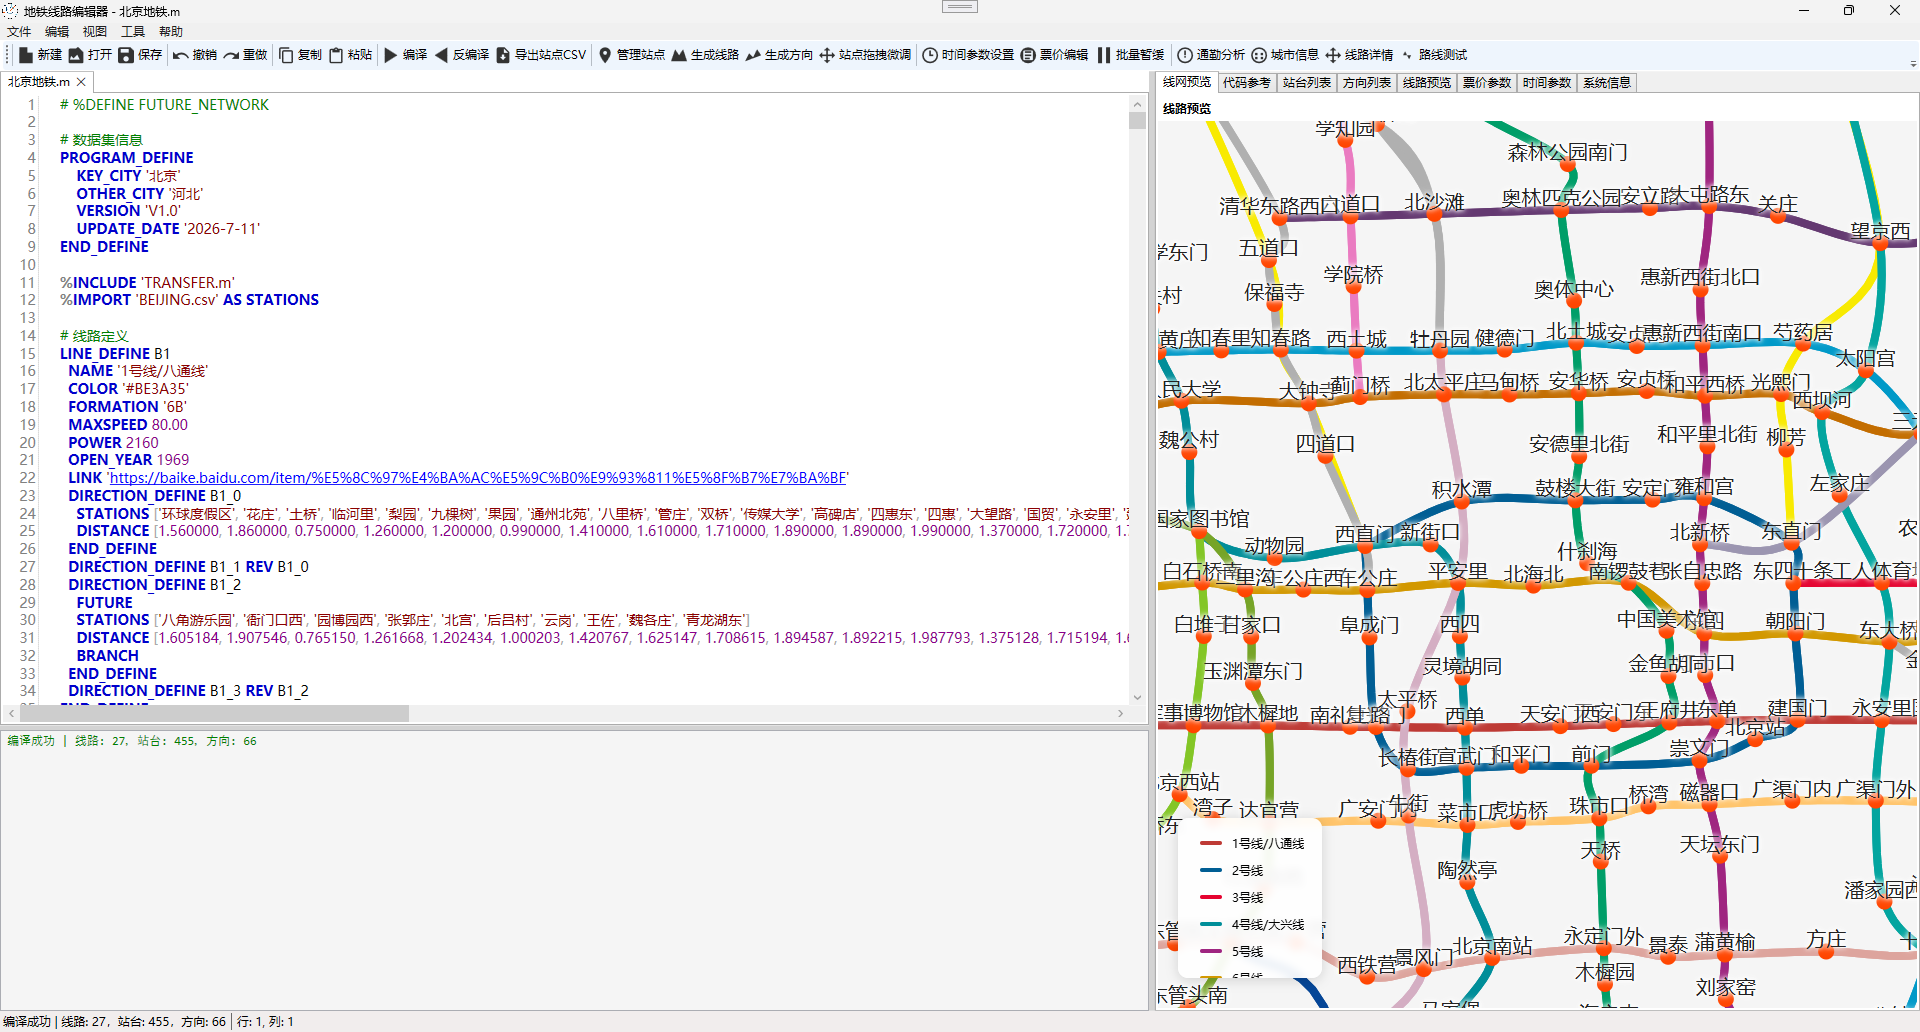
\includegraphics[width=0.8\textwidth]{figure/MetroLang.png}
	\caption{MetroEditor主界面截图（待插入）}
	\label{fig:app-metro-main}
\end{figure}

\subsubsection{核心功能}

\begin{enumerate}
	\item \textbf{MetroLang DSL}：领域特定语言描述地铁网络（站点、线路、方向、票价、换乘、运营参数等）。用户编写\texttt{.metro}文本文件，编译器将其编译为压缩的\texttt{.bmetro}二进制。
	\item \textbf{嵌入式导出}：将路网数据导出为专为资源受限设备设计的\texttt{.bin}二进制格式（零拷贝、大端序），或生成包含完整解析器的C语言代码（\texttt{metro\_parser.h/c} + \texttt{metro\_data.h}），支持多语言站名、预计算区间运行时间，适配STM32/FreeRTOS等平台。
	\item \textbf{通勤分析}：选择起点站，计算到所有站点的最优路径（距离、换乘、时间、票价、痛苦度），支持导出CSV。
	\item \textbf{设备同步}：通过TCP/UDP与Android客户端协同，一键推送地图到手机，实现路线查询、站点打卡、历史行程双向同步。
\end{enumerate}

\subsubsection{嵌入式导出的设计思路}

这是项目最贴近本书主题的部分。地铁线路数据通常包含数百个站点、数千个区间、复杂的票价规则和换乘信息。在嵌入式设备（如手持刷卡机、站内导引屏）上，不可能运行完整的JSON解析器或数据库引擎。

解决方案是：在PC端完成所有“重计算”，只把“查表”所需的数据结构导出为C代码或二进制：

\begin{itemize}
	\item 站点名称：主名与备用名分离存储，嵌入式端通过语言索引快速获取对应翻译；
	\item 区间运行时间：基于物理模型（编组、功率、限速、制动减速度）在PC端预先算好，嵌入式设备只需做整数加法即可完成路径搜索，无需浮点运算；
	\item 数据结构：强制大端序，支持零拷贝直接映射到结构体，无需解析。
\end{itemize}

导出的C代码示例如下（\texttt{metro\_data.h}）：

\begin{lstlisting}[style=c]
	/* 站点数量 */
	#define METRO_STATION_COUNT 128
	
	/* 站点名称表（支持多语言） */
	extern const char *metro_station_names[METRO_STATION_COUNT][2];
	
	/* 区间运行时间表（预计算，单位：秒） */
	extern const uint16_t metro_travel_time[METRO_STATION_COUNT][METRO_STATION_COUNT];
	
	/* 票价表（单位：分） */
	extern const uint16_t metro_fare[METRO_STATION_COUNT][METRO_STATION_COUNT];
	
	/* Dijkstra路径搜索（纯整数运算） */
	uint16_t metro_find_path(uint8_t start, uint8_t end, uint8_t *path, uint8_t max_depth);
\end{lstlisting}

这种“编译期完成重计算、运行期只查表”的思想，与正文第~\ref{ch:script-engine}~章“Python生成器在PC端完成文法分析，单片机只运行生成的C代码”如出一辙。

\begin{table}[htbp]
	\centering
	\caption{MetroEditor与正文各章的对应关系}
	\label{tab:app-metro-mapping}
	\begin{tabular}{lll}
		\toprule
		正文章节 & 对应功能 & MetroEditor中的实现 \\
		\midrule
		第~\ref{ch:command-parser}~章 & 命令解析 & MetroLang DSL的词法/语法解析器 \\
		第~\ref{ch:script-engine}~章 & 生成器思想 & .metro → C代码/二进制导出 \\
		第~\ref{ch:memory-alloc}~章 & 静态内存布局 & 零拷贝二进制结构体映射 \\
		第~\ref{ch:oop-in-c}~章 & 面向接口 & 嵌入式C解析器的统一API \\
		\bottomrule
	\end{tabular}
\end{table}


\section{塑料轮子哲学：一个贯穿始终的红线}

回顾这些项目，可以发现一条清晰的线索：

\begin{itemize}
	\item STC8H智能小车（2023）：用语音模块加蓝牙遥控，替代更复杂的自主导航方案——功能缩水但能跑；
	\item RK3588挑战杯项目（2025）：试图做“完整系统”，结果烂尾——画饼的代价；
	\item STM32H743+MaixCAM毕业设计（2026）：放弃ROS2，用条件域指令替代完整SLAM——塑料轮子策略的成功；
	\item SleepReminder（2026）：用三层守护进程对抗自己的熬夜冲动——直到发现“战胜自己太麻烦”才是最有效的“塑料轮子”；
	\item MetroEditor（2026）：用PC端重计算换取嵌入式端的轻量查表——一种“文明版”的塑料轮子。
\end{itemize}

作者在第~\ref{ch:about-author}~章里说过：“热爱可以等，交期不等。”这句话的背后，是对“塑料轮子”的深刻理解：它不是在否定更先进的技术方案，而是在承认“在有限的时间、有限的资源、有限的精力下，先交付一个可用的结果，比追求一个完美的方案更重要”。

这个附录里的每一个项目，都是这句话的注脚。
